\documentclass{article}
%packages
\usepackage{setspace}
\usepackage[T1]{fontenc}
\usepackage[utf8]{inputenc}
\usepackage[affil-it]{authblk}
\usepackage[margin=1in]{geometry}
\usepackage{amsmath,amssymb,amsthm}
\usepackage{mathabx}
\usepackage[usenames,dvipsnames,svgnames,table]{xcolor}
\usepackage{graphicx}
\usepackage{stmaryrd}
\usepackage{mathrsfs}
\usepackage{amsfonts}
\usepackage{enumitem}
\usepackage{dsfont}
\usepackage{bbold}
\usepackage{subcaption}
\usepackage{glossaries}
\usepackage{verbatim}
\usepackage[many]{tcolorbox}
\usepackage{tabulary}
\usepackage{booktabs}
\usepackage{tikz-cd}
\usepackage{tikz}
\usepackage{faktor}
\usepackage{xfrac} 
\usepackage{varwidth}
\usepackage{enumitem}
\usepackage{float}
%\usepackage{palatino}
\usepackage{framed} 
\usepackage{dirtytalk}
\usepackage{chngcntr}
\usepackage{tasks}
\usepackage{tabto}
\usepackage{import}
\usepackage{float}
\usepackage[pagewise]{lineno}

\usepackage{algorithm}
\usepackage{algpseudocode}
\usepackage{graphics}

%% Theorem definitions
\theoremstyle{plain}
\newtheorem{theorem}{Theorem}[section]
\newtheorem{proposition}[theorem]{Proposition}
\newtheorem{claim}[theorem]{Claim}
\newtheorem{lemma}[theorem]{Lemma}
\newtheorem{corollary}[theorem]{Corollary}
\newtheorem{conjecture}[theorem]{Conjecture}

\theoremstyle{definition}
\newtheorem{definition}{Definition}
\newtheorem{example}{Example}
\newtheorem{problem}{Problem}
\newenvironment{problem*}[1]
  {\renewcommand\theproblem{#1}\problem}
  {\endproblem}


\newtheorem{case}{Case}
\theoremstyle{remark}
\newtheorem{remark}[theorem]{Remark}
\renewcommand*{\proofname}{Solution}

\numberwithin{equation}{section}


%%%%%%blackboard letters
\newcommand{\bC}{\mathbb{C}}
\newcommand{\bN}{\mathbb{N}}
\newcommand{\bK}{\mathbb{K}}
\newcommand{\bP}{\mathbb{P}}
\newcommand{\bQ}{\mathbb{Q}}
\newcommand{\bR}{\mathbb{R}}
\newcommand{\bZ}{\mathbb{Z}}

%%%%%calligraphic commands%%%%

\newcommand{\cA}{\mathcal{A}}
\newcommand{\cB}{\mathcal{B}}
\newcommand{\cC}{\mathcal{C}}
\newcommand{\cF}{\mathcal{F}}
\newcommand{\cG}{\mathcal{G}}
\newcommand{\cI}{\mathcal{I}}
\newcommand{\cJ}{\mathcal{J}}
\newcommand{\cK}{\mathcal{K}}
\newcommand{\cL}{\mathcal{L}}



%%%%% some color macros  %%%%%

\newcommand{\tcr}[1]{\textcolor{red}{#1}}
\newcommand{\tcb}[1]{\textcolor{blue}{#1}}
\newcommand{\tcg}[1]{\textcolor{green}{#1}}
\newcommand{\tcc}[1]{\textcolor{cyan}{#1}}
\newcommand{\tcm}[1]{\textcolor{magenta}{#1}}
\newcommand{\tcp}[1]{\textcolor{purple}{#1}}

%%%%% derivative and laplace macros %%%%%

\newcommand{\der}[2][]{\frac{d#1}{d#2}}
\newcommand{\pder}[2][]{\frac{\partial#1}{\partial#2}}
\newcommand{\lt}[1]{\cL\{#1\}}
\newcommand{\displaylt}[1]{\cL\left\{#1\right\}}
\newcommand{\ilt}[1]{\cL^{-1}\{#1\}}
\newcommand{\displayilt}[1]{\cL^{-1}\left\{#1\right\}}

\newcommand{\SZ}[1]{\par \noindent
  \framebox{\begin{minipage}[c]{0.95 \textwidth}\color{purple} SUNNY'S NOTE:
      #1 \color{black}\end{minipage}}\par}

\newcommand{\MJ}[1]{\par \noindent
  \framebox{\begin{minipage}[c]{0.95 \textwidth}\color{purple} MASOUD'S NOTE:
      #1 \color{black}\end{minipage}}\par}

\title{Comparing Parent and Children Language Production}
\author{Sunny Zhou}
\affil{Department of Linguistics\\University of California, Davis}
\date{\today}


\begin{document}
\maketitle
\begin{abstract}
The production of words marks an important part of language development: some words develop before others. This staggered development of certain words, including over-generalization of grammatical rules or certain words, suggests how language is deeply connected to how we perceive the world. Specifically, the use of function words can tell us about how an individual processed the relationship and context between the content. In this study, we compare the word production frequencies of parents and children in recordings to parents and children interactions, highlighting what role function words play in the interactions. We show that parents and children follow the same product distribution (i.e. Zipf distribution).
\end{abstract}

\section{Introduction}

This study attempts to explore language developmental milestones through the word frequencies of parents and children. The goal of this study is to explore methods of using the statistical distribution of word production to analyze children's language development. Specifically, I claim that the development of function words signifies important developmental milestones such as in logic and entity recognition. In Section 3, I will go over the methods I used for gathering the data. Due to the nature of the study, much of this section will cover the calculation and plotting of the data, explaining my reasoning for why I plotted the data the way I did. In Section 4, I review observations from my graphs. Finally, in Section 5, I will discuss the implications of this data, the shortcomings of my methods, and what future research would strengthen the findings suggested.

\section{Background}
\subsection{Language Development}

Children’s developmental milestones in children ages 1 to 72 months have been well documented by psychologists and teachers. These milestones are observed through studies oillustrate the moments when children begin developing specific psychological and logical processes. Using these milestones and the age they occur at, we can get a picture of what is to be expected at each age. Each developmental phase is associated with respective language development (See Table~\ref{Tab:development}).

On the other hand, language development can be a useful tool to observe psychological development. The navigation through language can be a daunting task. Specifically, the development of grammar and the ability to determine grammatical categories of words is essential in learning a language. This implies the importance of parent-child interactions; the parents play a large role in what language the children are exposed to. There is a careful balance between using unfamiliar language and concepts to aid children's development. One example of children adding known information into sentences is through the use of definite and indefinite articles. Proper use of the words entails an understanding that definite articles imply that the entity introduced is old information, while the indefinite article signifies new information (\cite{clark2009first},339), reflecting this development.

A good example of the overuse of words is with simple categories such as negations and conjunctions. 

In studies on language acquisition, word frequency (content and function words) has been extended to determine an individual's language competency (\cite{feldman2019speech}, \cite{choi2018article},\cite{jasbi2020neg}). Since function words play such an important role in the structure of languages, the frequency trends of these words will ``properly" use them used to classify even more mastery of a language.

 

\subsection{Parents' Adaptation}

It should be obvious that children's lanague performance changes over time, depending on what concpets they develop. Hoever, little reserach has been done surround the parents. 

Although how do parents' performance adapt based on the child's language evolution? 

\subsection{Function Word Categories}
To start identifying what words signify, we first must establish the differences between words. That means establishing word categories. There are two categories of words: \emph{content words} and \emph{Function words}. \emph{Content words} define the who-what-where-how of the sentence (i.e. nouns, verbs, adjectives, adverbs, etc.). In the sentence ``The dog chewed on the bone," the content words tell us that there is two entities ``dog" and ``bone" related by the action of``chewed."

However, it is clear that something is missing semantically in this interpretation. For example, the word ``the" in front of ``dog" signifies that there is a specific dog being identified. Consider the previous sentence, ``The dog chewed on the bone." By manipulating the words ``on" and ``the," the sentence becomes ``the dog chewed with a bone."  Notice how the same content words are used in both sentences, but the relations between them change, yielding a semantically different sentence. These words, called \emph{function words} ``provide the ‘grammatical glue’ among the \emph{content words}"(\cite{pittphilsci16750}). Thus, typically, function words are described to be more 'grammatical' than 'content.'

The distinction between these two categories can be debated, arguing what it means to be 'content' or 'grammatical' (\cite{pittphilsci16750}). After all, what does it mean for something to hold 'content?' For the purposes of this study, 'grammar' words need to provide information that relates the entities and actions in a semantically significant way. Specifically, if the word can be removed and replaced by a null variable, such as 'a,' without losing grammatical information, then it is a grammar word. It is important to also mention that similar to how the content words category can be divided further into nouns, verbs, etc.., function words can as well. This splits the larger category into lexical and grammatical categories. There are different categories of function words that will be focused on throughout this study. Examples of these categories can be seen in Table~\ref{Tab:category}.

There is a whole separate issue of whether the children understand, or implement, the language correctly. In this study, I ignored this, in order to focus on frequencies and language production. 

\subsection{Zipf Distribution}
The first part of this study compares the word production frequency of children and parents. It is known that all word frequencies follow a probability density function called Zipf Distribution (\cite{tullo2003zipf}). In this distribution, words are ranked from most-occurring (r=1) to least-occurring (r=n) and follow roughly a $\frac{1}{r}$ proportion, where $r$ is the frequency rank of the word.

%%%%%%%%%%%%%%%%%%%%%%%%%%%%%%%%%%%%%%%%%%%%%%%%%%%%%

\section{Study 1}
\subsection{Methods}
The CHILDES TalkBank database was chosen for its expansive wealth of data. It compiles many studies on child-parent interactions, many of which follow longitudinal studies. Since the amount of data in the database is extensive, this study is focused on English speakers. To ensure this, I only collected data from the North American and United Kingdom collections of the CHILDES TalkBank. In particular, there are 15,824,850 token observations, from 2,005 unique participants (i.e. 794 children and 1211 parents). Since the data were taken from longitudinal studies, many of the children were surveyed multiple times at different ages. This study is interesting in tracking the change in the language development of the children, thus it is important to consider the same children at different ages as different participants. With this criteria, there were, instead, 5,851 participants (i.e. 2713 children and 3138 parents). The children ranged from 3.460030 months to 71.95425 months, with most participants being around 24 months old (see Figure \ref{fig:ages}). 

To collect the data needed for this study, I utilized the R package \emph{childesr} to access CHILDES TalkBank database \cite{macwhinney2000childes} to sample the function word usage in children. The code is an adaptation of Jasbi's code (\cite{masoud2022git}). For the purposes of the study, content words were grouped into one category. The primary reason the \emph{childesr} package was chosen was for its ease of use when presenting the data in a data frame in R. Utterances were annotated for the type of sentence (declarative, interrogative, imperative) and 13 syntactic categories (see Table~\ref{Tab:category}). 

I modeled my data analysis after \cite{jasbi2020neg}, where to observe whether children have achieved a typical production of a word, I compared the performance of children to the performance of parents. Since the goal is to observe at what age children develop certain vocabulary, alluding to developmental milestones, the data was binned by the target child's age. There were significantly more utterances produced by parents than children (). In the case of parents, this represents what age of the child was being interacted with. This works under the assumption that parent performance is consistent and typical, so children's frequencies ``meeting" the parents' frequencies means that they have developed to a typical level. To achieve this, occurrences of tokens were counted and grouped by the speaker type and participating child's age. It is important to note that the same distribution would appear if raw frequencies were plotted; however, since children produce significantly less speech than parents, graphing their raw frequencies together would not represent the data properly, underrepresenting the children's language. 
\subsection{Results}

By graphing against the participating child's age, the aim was to observe how parents adapted their speech to the children's ages. Considering how language is connected to thought, by plotting function word frequencies in relation to children's ages can illustrate these advancements. My first question is focused on the probability density of parent and child word production frequencies. Specifically, whether or not children follow a similar Zipf distribution. I split the corpus into two groups (parents and children tokens) and counted the occurrences of each token that appeared in the corpus. I then plotted the occurrences of each token, independent of the ages of the target child. This gave me a raw frequency graph (see Figure~\ref{fig:general_raw}). The number of occurrences was divided by the total number of tokens to give a relative frequency (see Figure~\ref{fig:general_rf}). This was plotted on a log-log graph to better observe the characteristics of the plot and compare it with the Zipf distribution. 

%%%%%%%%%%%%%%%%%%%%%%%%%%%%%%%%%%%%%%%%%%%%%%%%%%%%%
\subsection{Results}
For the second question, we need to compare trends of the word category relative frequencies (Figure~\ref{fig:category}). We notice that the trend of parent and child language production is not the same for all categories: in some of the categories they intersect immediately, in some they take a few years, and in others, they seem to travel parallel. In particular, we see that in logical connectives (Figure~\ref{fig:log}), the category that contains \emph{no, not, n’t}, the children ``catch" up to the parents by 13 months. In quantity (Figure~\ref{fig:quant}), such as \emph{more, less, much}, children exceed parents' production at 12 months, but then ``adjust" to parent productions at 36 months. While in ordinals (Figure~\ref{fig:ord}), such as \emph{first, second, third, fourth}, children never reach their parents. On the other hand, although depending on the categories, children meet, or exceed, the production of parents, we see that many of the graphs follow a pattern of children starting with low production and then matching parent production eventually. 

This pattern can be observed, as well, when looking at specific word productions (Figure~\ref{fig:word}). The most fascinating example of this is when comparing the definite and indefinite articles ``the" and ``a." Notice how children exceed parents for ``a" at 16 months, but then adjust at 36 months, which is around the same ``the" production meets parent levels. Additionally, when comparing, the words ``you" and ``I" (Figure~\ref{fig:i_you}), we notice that once children exceed parent productions of ``I" at 16 months, they never adjust back to parent levels. Whereas, children never exceed parent levels for ``you."

\subsection{Conclusion}
\section{Study 2}

\subsection{Methods}
This study utilizes the same database as the previous one. However instead of grouping the children and parents by the age of the target child, there was not distinction made. This allows me to observe the overall trend of language production. 

Like previous studies, to observe the Zipf distribution of function words, I calculated the relative frequencies of each word grouped by speaker type (i.e. parent or child). 
To answer my question of whether the relative and log frequencies of children and parent language. As shown in Figure~\ref{fig:general_raw}, the statistical distribution of (a) the children's frequency graphs matches that of (b) the parents'. In fact, both graphs follow a distribution similar to Zipf distribution. This is supported further by Figure~\ref{fig:general_log}, showing a fairly linear relationship between frequency rank and frequency on a log-log graph, until it drops off at around frequency rank 80. Focusing on the ranking 1-80 in Figure~\ref{fig:log}, we see that the slope is around $1/16$ for both children and parents, supporting that they both have the same form.
\subsection{Conclusion}

%%%%%%%%%%%%%%%%%%%%%%%%%%%%%%%%%%%%%%%%%%%%%%%%%%%%%
\section{Discussion}

\subsection{General Word Frequencies of Participants}
It has been established that adult language production follows a Zipf distribution, this doesn't come as a surprise. However, as mentioned previously, the vocabulary available to children is vastly different from that of adults; thus, it is surprising that children match this distribution. In other words, this show empirically that children's word production follows the same distribution as parents, despite producing less speech in general. 

Taking a closer look at the specific tokens in the general graphs, we observe similar results to the general graphs. In Figure~\ref{fig:general_raw}, we can see that the most frequent grammatical category, for both parents and children, are content words, as signified by the key. Specifically, the top occurring words are ``I" and ``you," respectively. This result can be explained by the nature of the analyzed corpus. In many of the child-parent interactions found in TalkBank, the parent is prompting the child by directing questions, which are followed by an answer by the child. The nature of this type of conversation involves one party talking about the other, and the other party responding about themselves. This implies a ``you" and a ``I" split in productions. Additionally, it comes as no surprise that the next two words for both are ``the" and ``a." 

\subsection{Language Developmental Trend}
On the other hand, Figure~\ref{fig:category} compares production trends of parents and children. As previously noted, the patterns between ``the" and ``a" are an important one. A possible explanation of this is the over-generalization of the indefinite article. This normalization of ``a"'s usage suggests a change in the child's understanding of what a definite entity is, hinting at the suggested implications in the introduction. The overuse of words is something that has previously been observed in other words, such as negations \cite{jasbi2020neg}. The justified removal of these occurrences may be necessary to observe more general trends.

In these findings, there are some places for future improvements. It is important to point out how ``production" is used interchangeably with ``relative frequency." Typically, ``production" refers to the raw frequencies: the actual total occurrence of each word. While the ``relative frequency" compares to production of certain words to the total. However, we know that children have a limited vocabulary and produce less language in general. Because of this, these concepts have been equated to ``normalize" and properly compare the two groups. It has also been noted, by others, that some tokens, such as slang, were mis-categorized as ``other" or ``content." A careful inspection of all of the tokens is necessary to filter out these errors, which led to the trend observed in Figure~\ref{fig:con}.

\subsection{Future Research}
Similar methods can also be applied to adult interactions, such as television genres, to measure specialized diction. Future research could include the implementation of natural language models used to infer lexical contexts based on the distribution of function words. This could also have an impact on how we can interpret intent and truthfulness and better understand the deceitful language from media. It would also be interesting to generalize these methods to other languages, such as ones that do not distinguish articles, such as Chinese. 

%%%%%%%%%%%%%%%%%%%%%%%%%%%%%%%%%%%%%%%%%%%%%%%%%%%%%
\bibliographystyle{apalike} 
\bibliography{biblio}

\section*{Acknowledgements}
Special thanks to Dr. Masoud Jasbi for mentoring me during this project.


\section*{Appendix}
\begin{figure}[H]
    \centering
    \includegraphics[width=\textwidth]{general_plots/age.png}
    \caption{This figure shows the distribution of participants at each age.}
    \label{fig:ages}
\end{figure}

    \begin{table}[H]
    \resizebox{\textwidth}{!}{\begin{tabular}[width=\textwidth]{|p{8cm}|p{8cm}|}
    \hline
        \rowcolor{LightGray}
        Category & Examples \\
                \hline
        Logical Connectives & no, not, n't, and, or, if, nor\\
        \hline
        Quantifiers & none, some, each, every, all, most, few, many, several, a few, both, everyone, someone, somebody, everybody, nonone, everything, something, nowhere, somewhere, everywhere\\
                \hline
        Comparative Quantity & more, less, much\\
                \hline
        Numerals & numbers: one, two, three, four, five, six, seven, eight, nine, ten; ordinals: first, second, third, fourth fifth, last\\
                \hline
        Modals & can, could, need, may, might, should, ought, must, maybe, perhaps, shall\\
                \hline
        Negative Polarity Items & any, anyone, anything, anyhow, anywhere, anything, anyway, ever, yet\\
                \hline
        Definiteness and Demonstratives & Definite: the, a, an; Demonstratives: this, that, these, those\\
                \hline
        Temporals &Quantifiers:  always, usually, seldom, never, sometimes, now, often, once; Connectives: when, while, after, before, then, until, since, whenever, during\\
                \hline
        Interrogatives & who, when, what, whose, where, how, why, whom\\
                \hline
        Locatives & on, in, out, up, down, under, above, below, along, over, behind, across, beside, between, beyond, inside, outside, into, near, onto, toward\\
                \hline
        Causal Connectives & because, therefore\\
                \hline
        Contrast Connectives & but, although\\
                \hline
        Additives & again, too, also, another, other, others, still\\
                \hline
        Focus Particles & even, only, indeed\\
                \hline
        Other & either, neither, whether as, else, almost, already, except, for, from, instead, same, different, such, with, without, about, by, very\\
                \hline
    \end{tabular}}
    \caption{A list of the labeled category and which tokens were to the category.}
    \label{Tab:category}
    \end{table}

\begin{figure}[H]
\begin{subfigure}[b]{0.5\textwidth}
    \centering
    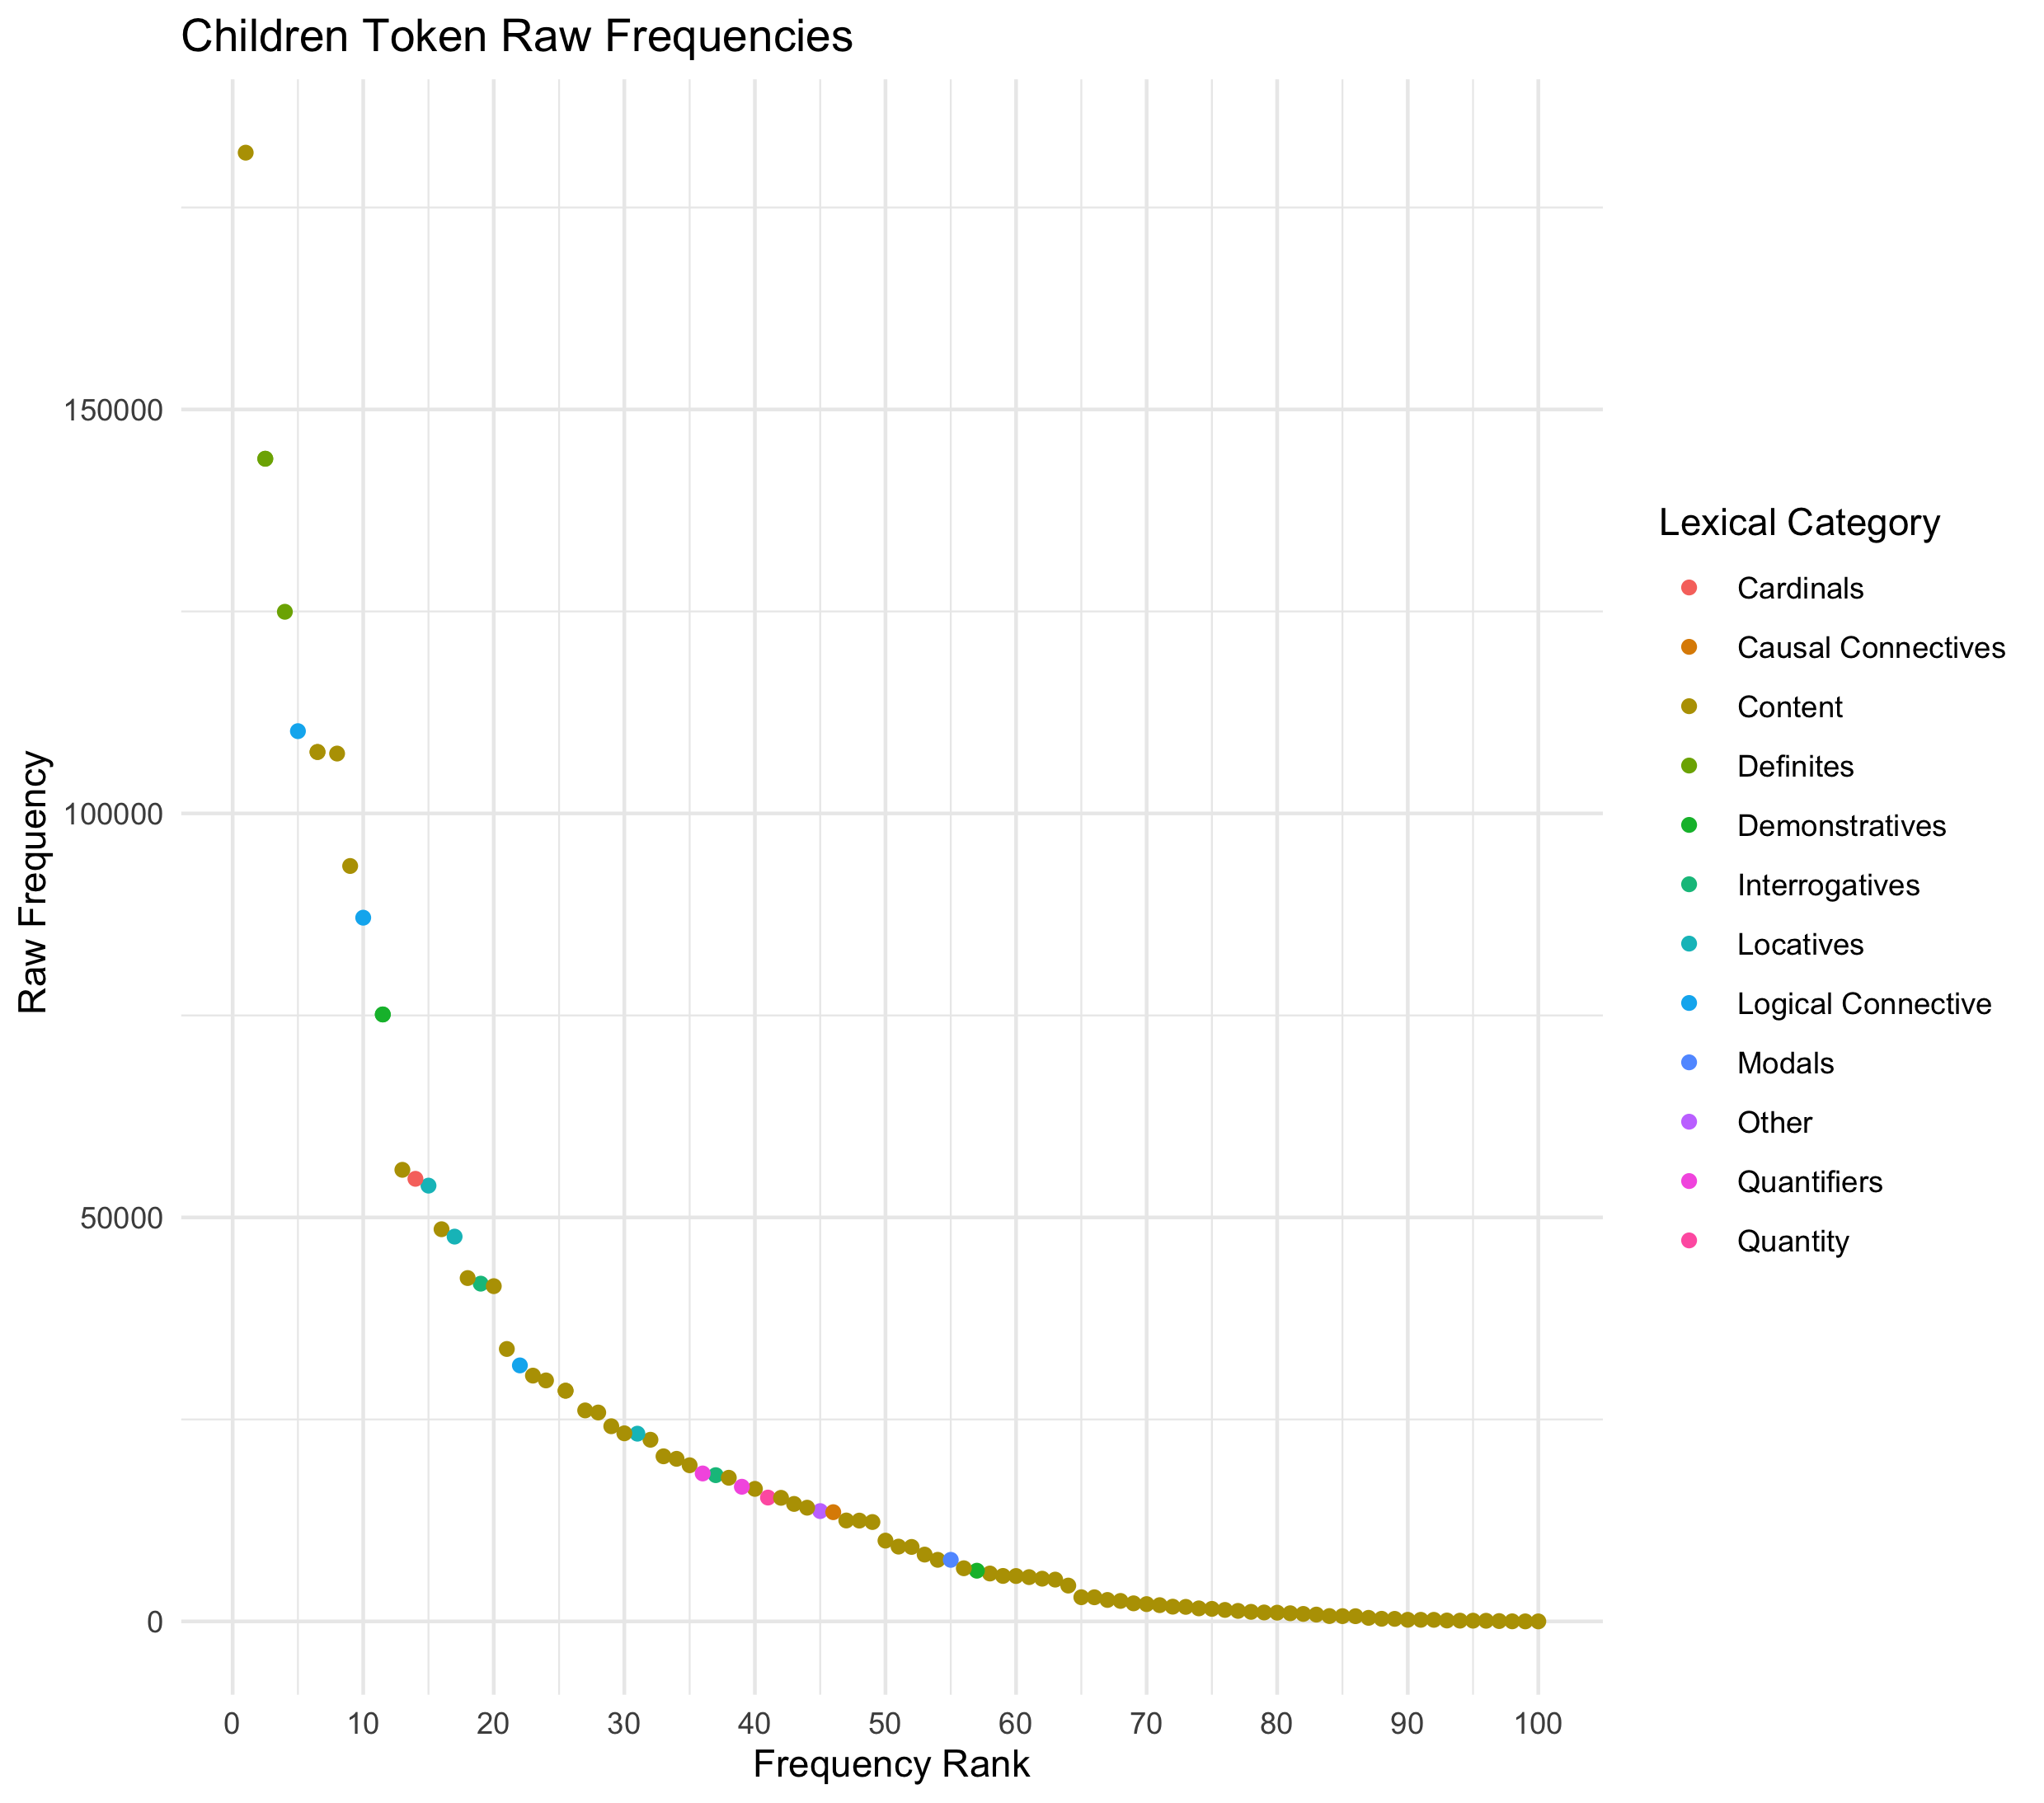
\includegraphics[width=\textwidth]{general_plots/child_general.png}
\caption{}
    \label{fig:child_raw}
\end{subfigure}
\hfill
\begin{subfigure}[b]{0.5\textwidth}
\centering
    \includegraphics[width=\textwidth]{general_plots/parents_general.png}
\caption{}
    \label{fig:parent_raw}
\end{subfigure}
   \caption{These graphs show the raw token frequencies with frequency rank on the x-axis and relative frequency on the y-axis: children (left) and parents (right).}
    \label{fig:general_raw}
\end{figure}

\begin{figure}[H]
\begin{subfigure}[b]{0.5\textwidth}
    \centering
    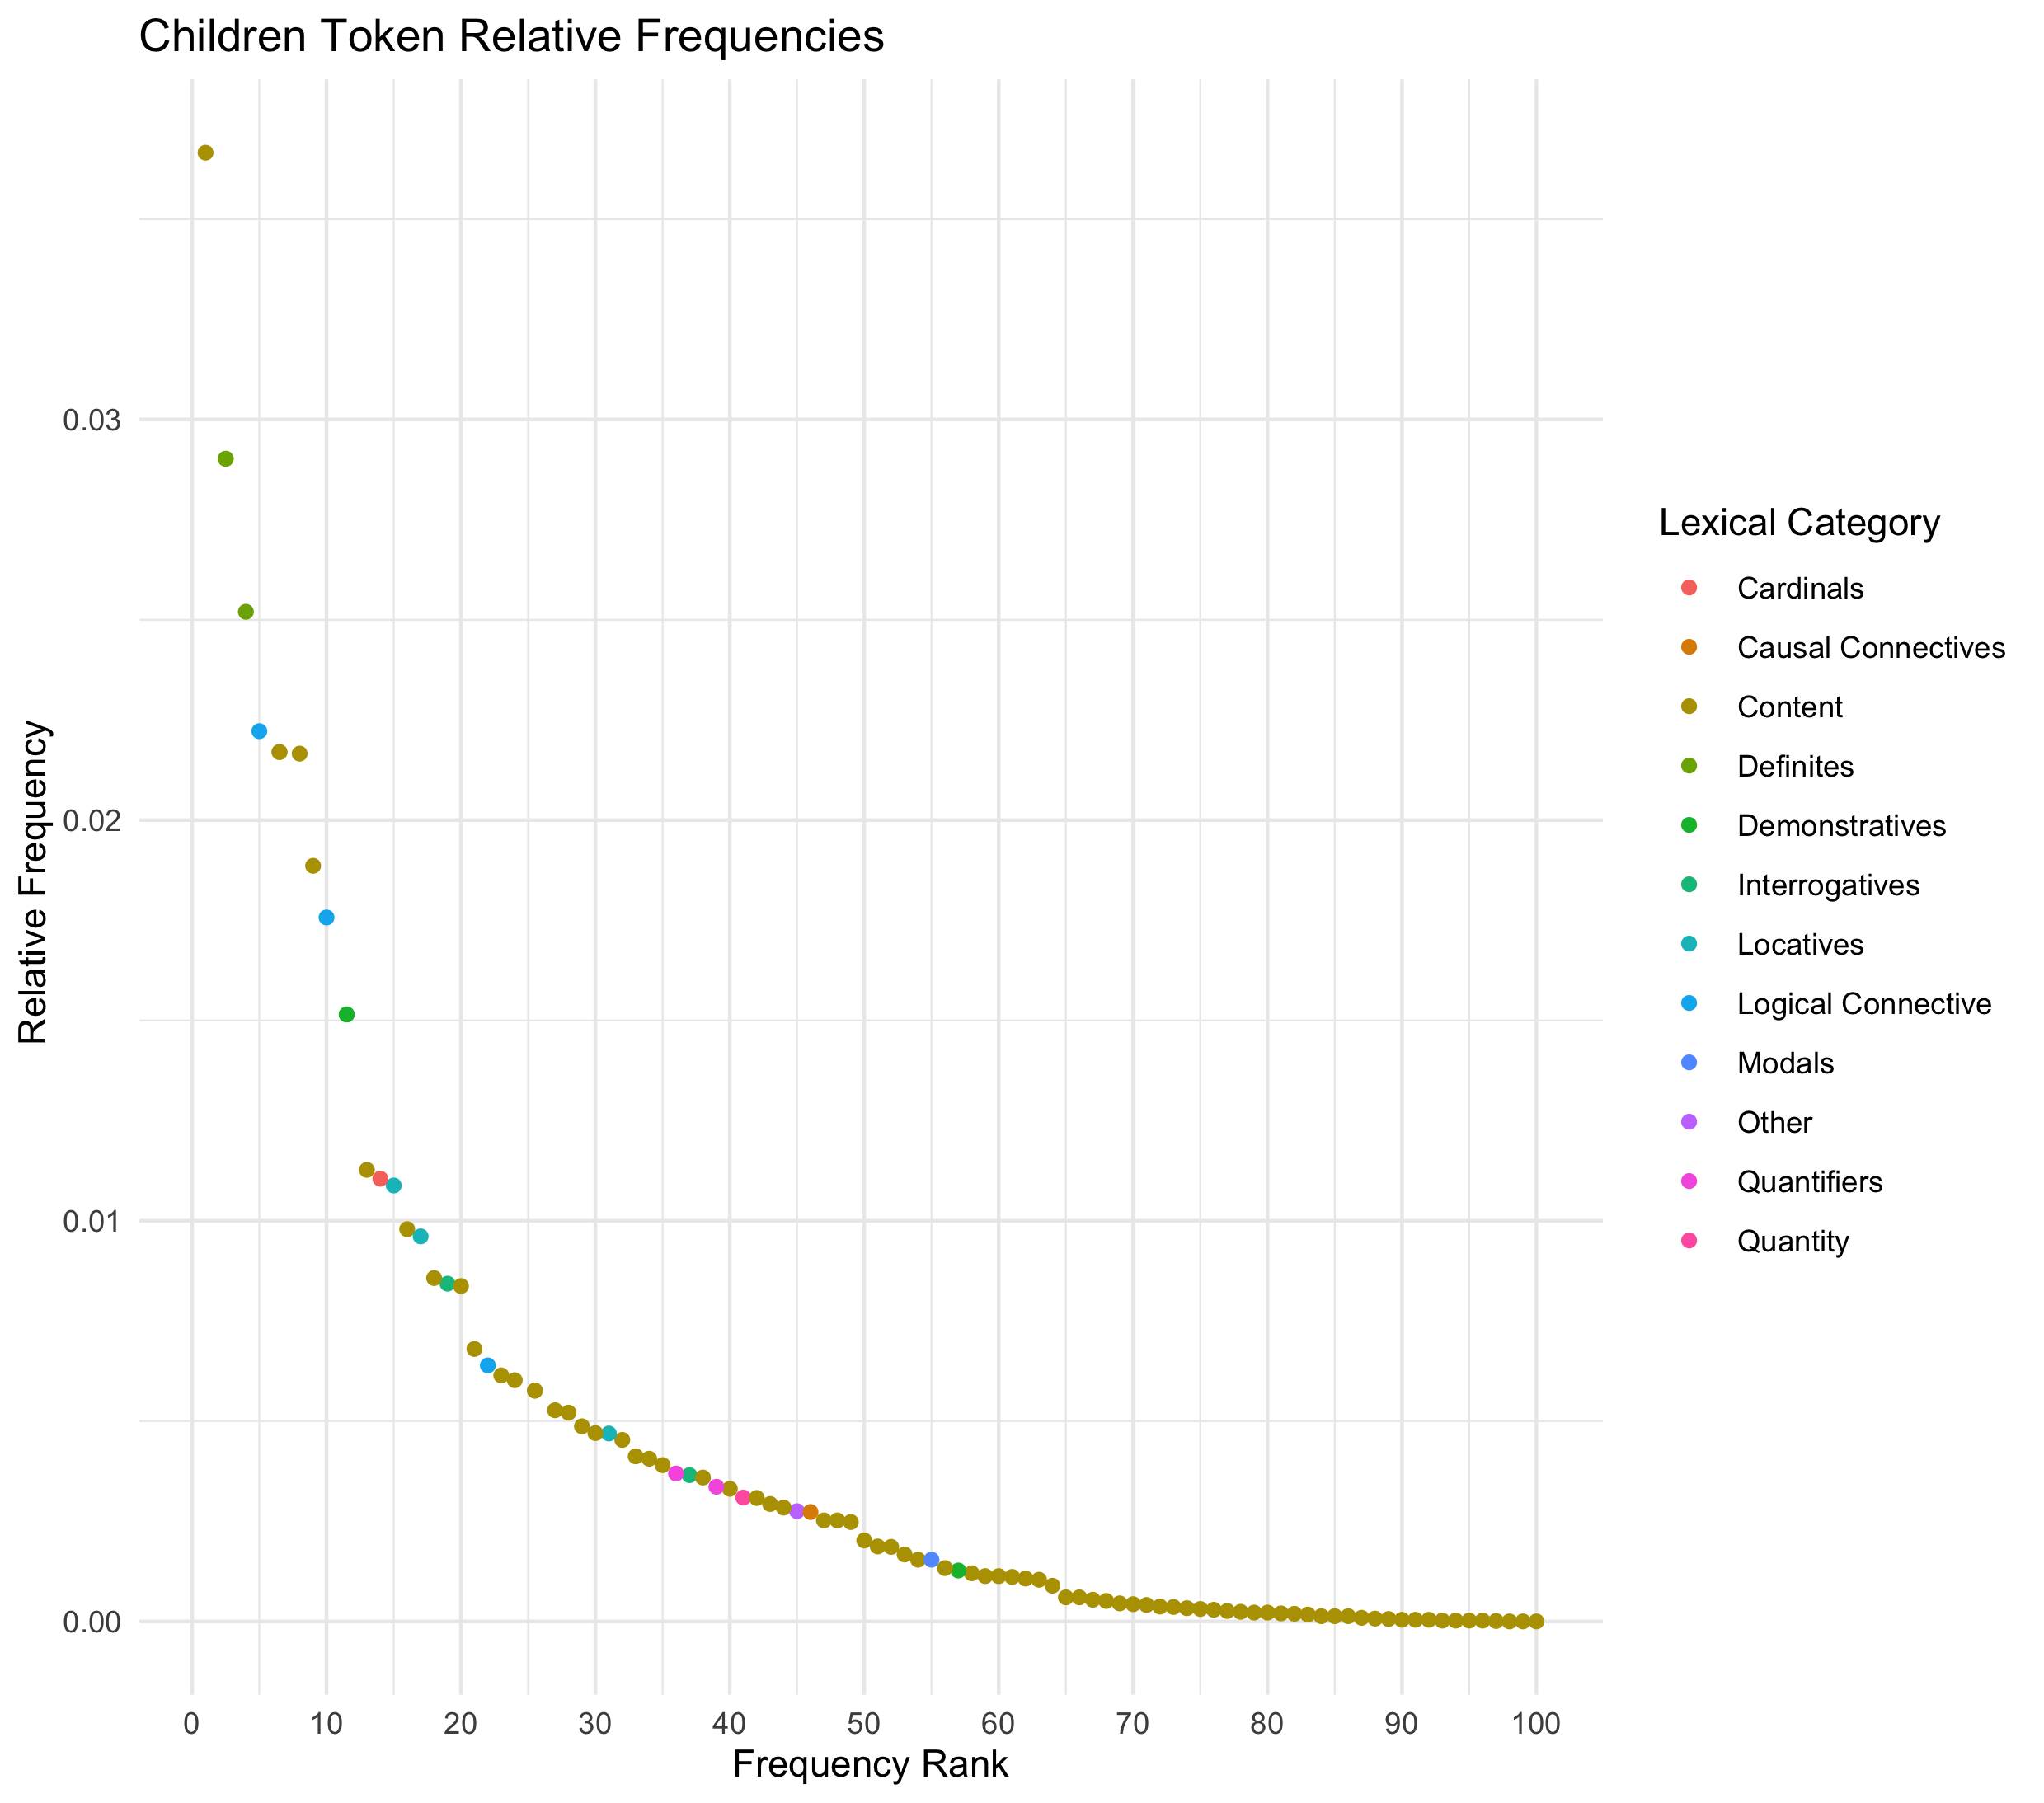
\includegraphics[width=\textwidth]{general_plots/child_general_rf.png}
\caption{}
    \label{fig:child_rf}
\end{subfigure}
\hfill
\begin{subfigure}[b]{0.5\textwidth}
\centering
    \includegraphics[width=\textwidth]{general_plots/parents_general_rf.png}
\caption{}
    \label{fig:parent_rf}
\end{subfigure}
   \caption{These graphs show the relative token frequencies with frequency rank on the x-axis and relative frequency on the y-axis: children (left) and parents (right).}
    \label{fig:general_rf}
\end{figure}

\begin{figure}[H]
\begin{subfigure}[b]{0.5\textwidth}
    \centering
    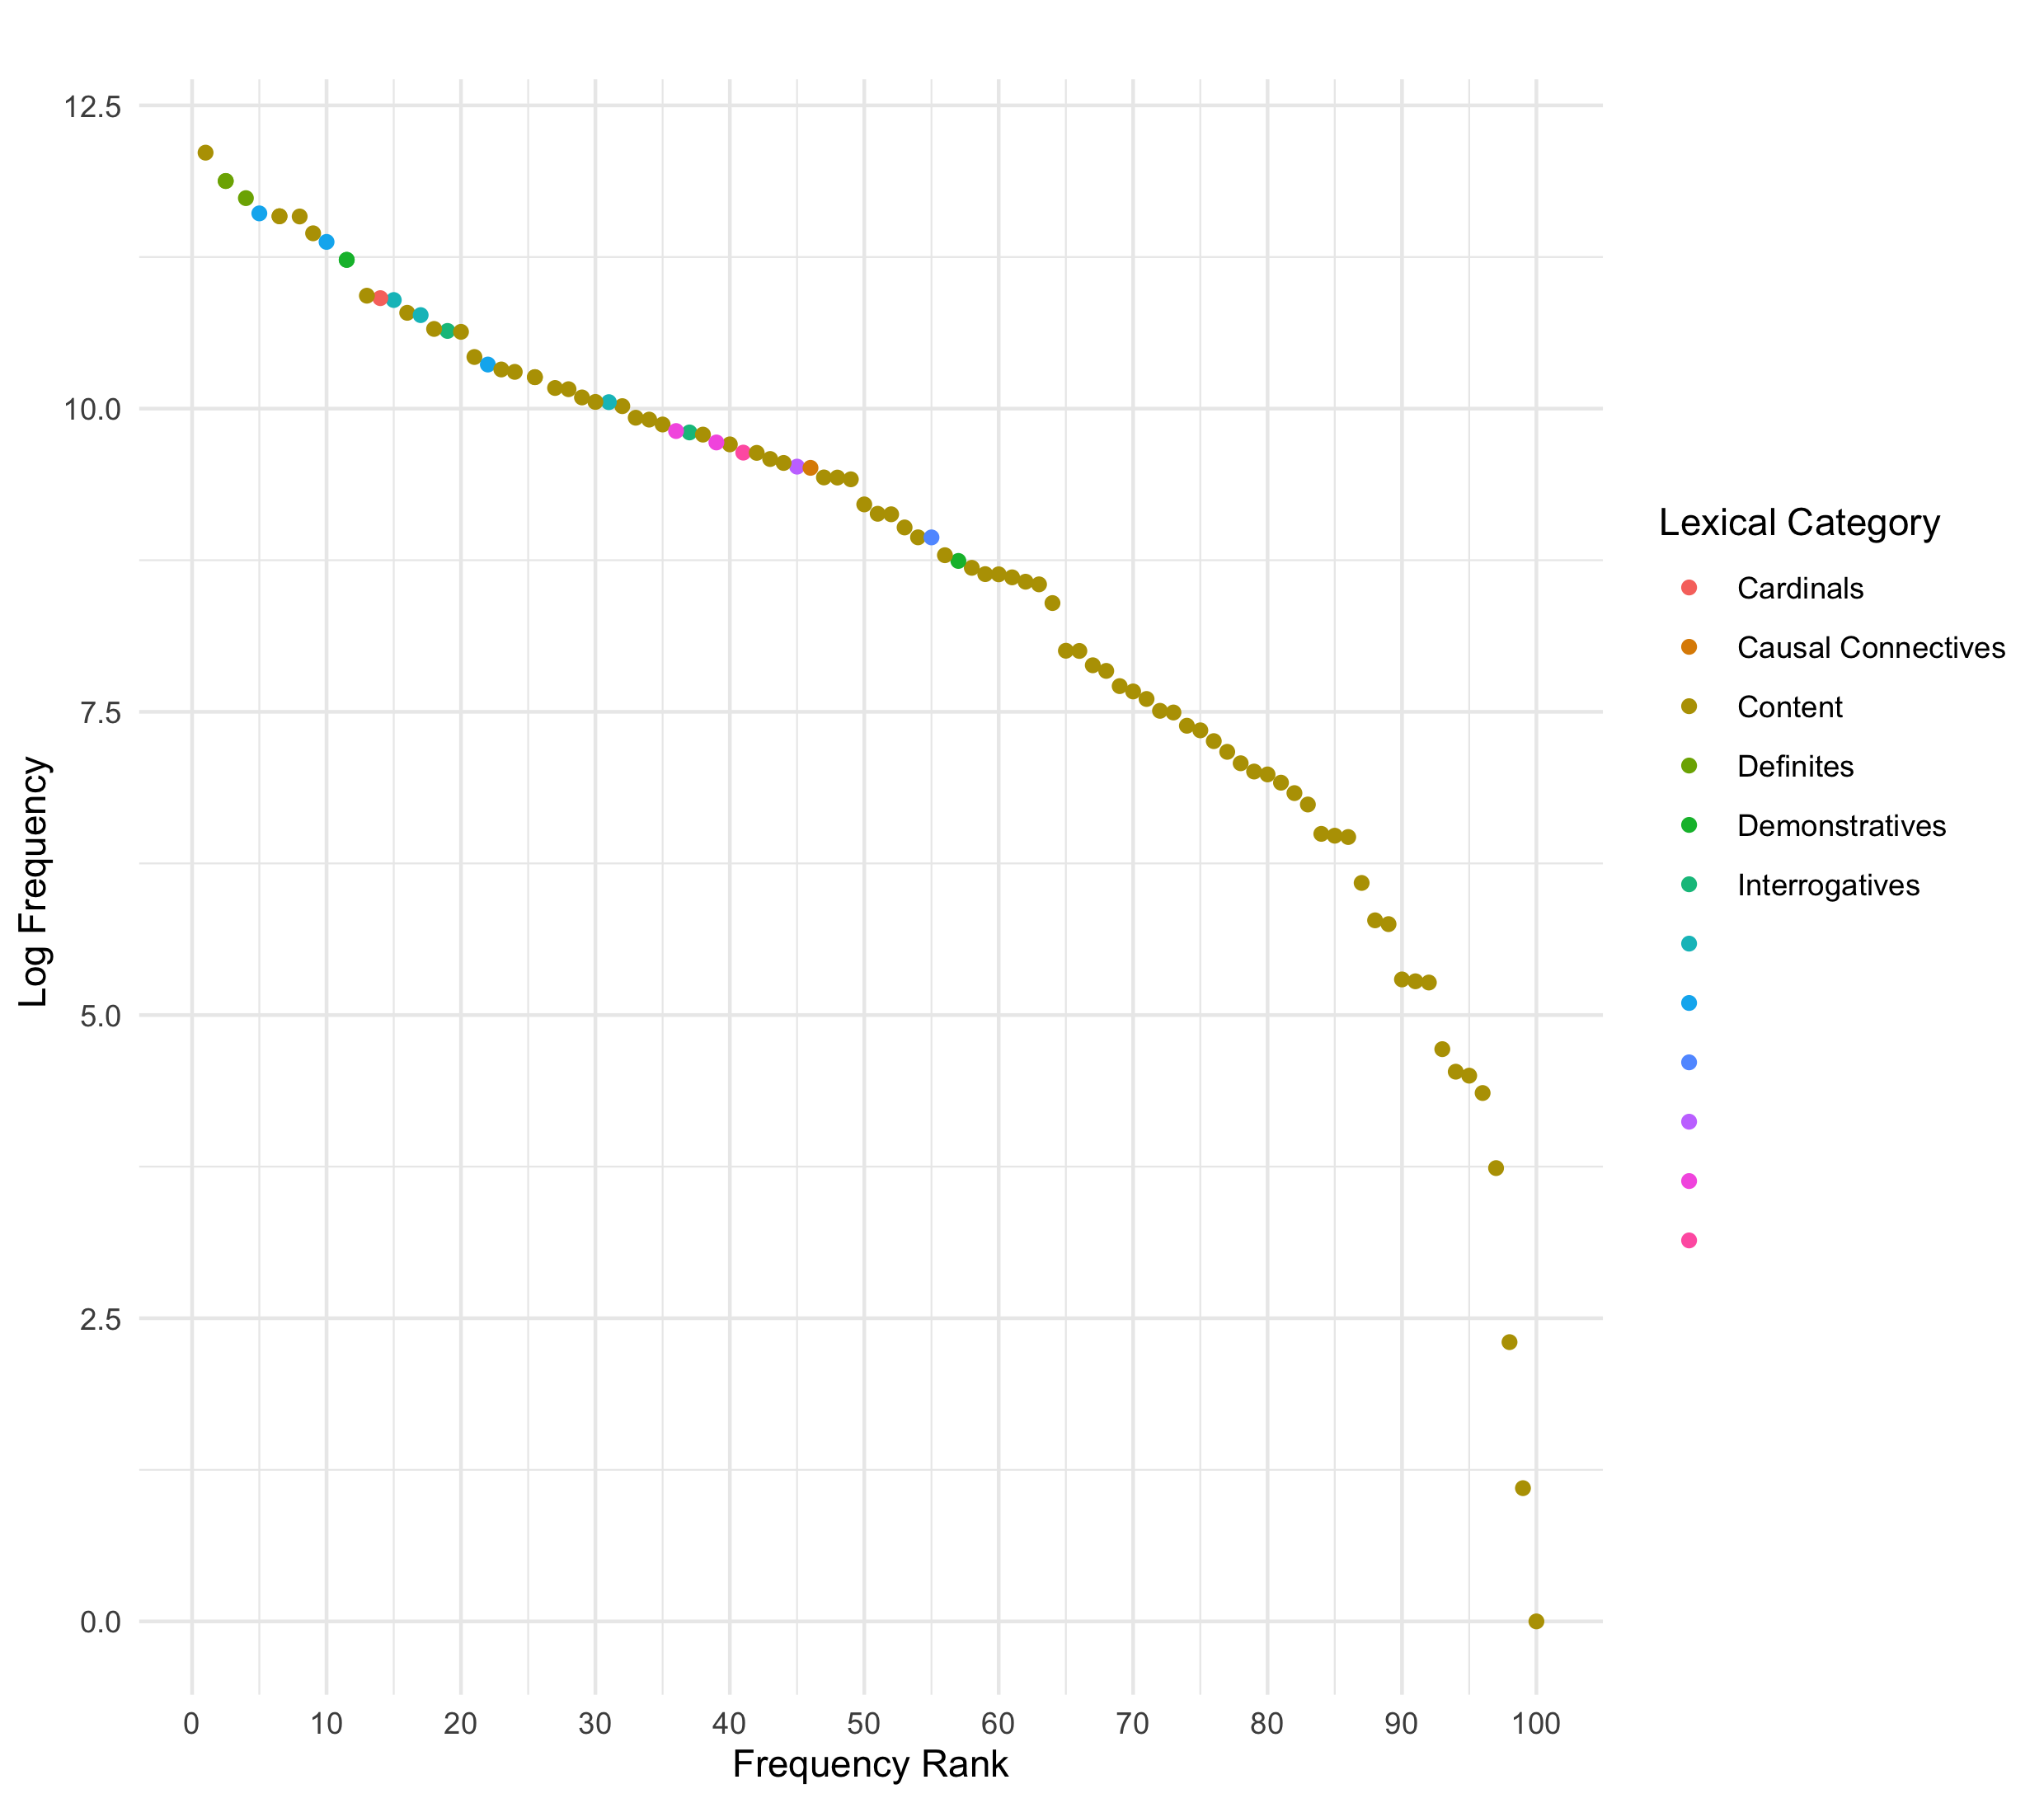
\includegraphics[width=\textwidth]{general_plots/child_general_logf.png}
\caption{}
    \label{fig:child_log}
\end{subfigure}
\hfill
\begin{subfigure}[b]{0.5\textwidth}
\centering
    \includegraphics[width=\textwidth]{general_plots/parents_general_log.png}
\caption{}
    \label{fig:parent_log}
\end{subfigure}
   \caption{These graphs show the relative token frequencies on a log-log graph with frequency rank on the x-axis and relative frequency on the y-axis: children (left) and parents (right).}
    \label{fig:general_log}
\end{figure}

\begin{figure}
\begin{subfigure}[b]{0.3\textwidth}
    \centering
    \includegraphics[width=\textwidth]{category_plots/Additives.png}
    \caption{}\label{fig:add}
\end{subfigure}
\hfill
\begin{subfigure}[b]{0.3\textwidth}
    \centering
    \includegraphics[width=\textwidth]{category_plots/Cardinals.png}
    \caption{}\label{fig:card}
\end{subfigure}
\hfill
\begin{subfigure}[b]{0.3\textwidth}
    \centering
    \includegraphics[width=\textwidth]{category_plots/Causal Connectives.png}
    \caption{}\label{fig:causal}
\end{subfigure}
\hfill
\begin{subfigure}[b]{0.3\textwidth}
    \centering
    \includegraphics[width=\textwidth]{category_plots/Content.png}
    \caption{}\label{fig:con}
\end{subfigure}
\hfill
\begin{subfigure}[b]{0.3\textwidth}
    \centering
    \includegraphics[width=\textwidth]{category_plots/Contrast Connectives.png}
    \caption{}\label{fig:connect}
\end{subfigure}
\hfill
\begin{subfigure}[b]{0.3\textwidth}
    \centering
    \includegraphics[width=\textwidth]{category_plots/Definites.png}
    \caption{}\label{fig:def}
\end{subfigure}
\hfill
\begin{subfigure}[b]{0.3\textwidth}
    \centering
    \includegraphics[width=\textwidth]{category_plots/Demonstratives.png}
    \caption{}\label{fig:demon}
\end{subfigure}
\hfill
\begin{subfigure}[b]{0.3\textwidth}
    \centering
    \includegraphics[width=\textwidth]{category_plots/Focus Particles.png}
    \caption{}\label{fig:focus}
\end{subfigure}
\hfill
\begin{subfigure}[b]{0.3\textwidth}
    \centering
    \includegraphics[width=\textwidth]{category_plots/Interrogatives.png}
    \caption{}\label{fig:int}
\end{subfigure}
\hfill
\begin{subfigure}[b]{0.3\textwidth}
    \centering
    \includegraphics[width=\textwidth]{category_plots/Locatives.png}
    \caption{}\label{fig:loc}
\end{subfigure}
\hfill
\begin{subfigure}[b]{0.3\textwidth}
    \centering
    \includegraphics[width=\textwidth]{category_plots/Logical Connective.png}
    \caption{}\label{fig:log}
\end{subfigure}
\hfill
\begin{subfigure}[b]{0.3\textwidth}
    \centering
    \includegraphics[width=\textwidth]{category_plots/Modals.png}
    \caption{}\label{fig:mod}
\end{subfigure}
\hfill
\begin{subfigure}[b]{0.3\textwidth}
    \centering
    \includegraphics[width=\textwidth]{category_plots/NPI.png}
    \caption{}\label{fig:npi}
\end{subfigure}
\hfill
\begin{subfigure}[b]{0.3\textwidth}
    \centering
    \includegraphics[width=\textwidth]{category_plots/Ordinals.png}
    \caption{}\label{fig:ord}
\end{subfigure}
\hfill
\begin{subfigure}[b]{0.3\textwidth}
    \centering
    \includegraphics[width=\textwidth]{category_plots/Other.png}
    \caption{}\label{fig:other}
\end{subfigure}
\hfill
\begin{subfigure}[b]{0.3\textwidth}
    \centering
    \includegraphics[width=\textwidth]{category_plots/Quantifiers.png}
    \caption{}\label{fig:quant}
\end{subfigure}
\hfill
\begin{subfigure}[b]{0.3\textwidth}
    \centering
    \includegraphics[width=\textwidth]{category_plots/Quantity.png}
    \caption{}\label{fig:num}
\end{subfigure}
\hfill
\begin{subfigure}[b]{0.3\textwidth}
    \centering
    \includegraphics[width=\textwidth]{category_plots/Temporal Quantifiers.png}
    \caption{}
    \label{fig:temp}
\end{subfigure}
\caption{These plots show the category usage relative frequency for each grammatical category. Each graph contains both parent and child trends, where the x-axis represents the child age bin being spoken to and the child age bin speaking, respectively. The y-axis represents the relative frequency of the category in relation to the total token production in the age bin.}
    \label{fig:category}
\end{figure}

\begin{figure}
    \centering
    \begin{subfigure}[b]{0.3\textwidth}
        \includegraphics[width=\textwidth]{word_plots/a.png}
        \label{fig:a}
    \end{subfigure}
    \begin{subfigure}[b]{0.3\textwidth}
        \includegraphics[width=\textwidth]{word_plots/and.png}
        \label{fig:and}
    \end{subfigure}
    \begin{subfigure}[b]{0.3\textwidth}
        \includegraphics[width=\textwidth]{word_plots/do.png}
        \label{fig:do}
    \end{subfigure}
    \begin{subfigure}[b]{0.3\textwidth}
        \includegraphics[width=\textwidth]{word_plots/i.png}
        \label{fig:i}
    \end{subfigure}
    \begin{subfigure}[b]{0.3\textwidth}
        \includegraphics[width=\textwidth]{word_plots/in.png}
        \label{fig:in}
    \end{subfigure}
    \begin{subfigure}[b]{0.3\textwidth}
        \includegraphics[width=\textwidth]{word_plots/is.png}
        \label{fig:is}
    \end{subfigure}
    \begin{subfigure}[b]{0.3\textwidth}
        \includegraphics[width=\textwidth]{word_plots/it.png}
        \label{fig:it}
    \end{subfigure}
    \begin{subfigure}[b]{0.3\textwidth}
        \includegraphics[width=\textwidth]{word_plots/no.png}
        \label{fig:no}
    \end{subfigure}
    \begin{subfigure}[b]{0.3\textwidth}
        \includegraphics[width=\textwidth]{word_plots/on.png}
        \label{fig:on}
    \end{subfigure}
    \begin{subfigure}[b]{0.3\textwidth}
        \includegraphics[width=\textwidth]{word_plots/that.png}
        \label{fig:that}
    \end{subfigure}
    \begin{subfigure}[b]{0.3\textwidth}
        \includegraphics[width=\textwidth]{word_plots/that's.png}
        \label{fig:thats}
    \end{subfigure}
    \begin{subfigure}[b]{0.3\textwidth}
        \includegraphics[width=\textwidth]{word_plots/the.png}
        \label{fig:the}
    \end{subfigure}
    \begin{subfigure}[b]{0.3\textwidth}
        \includegraphics[width=\textwidth]{word_plots/this.png}
        \label{fig:this}
    \end{subfigure}
     \begin{subfigure}[b]{0.3\textwidth}
        \includegraphics[width=\textwidth]{word_plots/you.png}
        \label{fig:you}
    \end{subfigure}
    \begin{subfigure}[b]{0.3\textwidth}
        \includegraphics[width=\textwidth]{word_plots/your.png}
        \label{fig:your}
    \end{subfigure}
    \caption{These are the graphs of relative frequencies, based on the participating child's age bin, of the specific words.}
    \label{fig:word}
\end{figure}






\end{document}
